% reset section counter
\setcounter{section}{0}

\metadata{15}{Tianyu Du, Xin Lu and Soham Sinha}{Mar 8th, 2021}

\sec{Review and overview}

In the last lecture, we finished off our discussion of algorithmic regularization. In a simplified setting, we proved that gradient descent on the empirical loss $\empL$ with a bounded number of iterations gives a solution $\widehat\beta$ that is close to the true solution $\beta^\star$.

In this lecture, we switch gears and talk about \textit{online learning} and \textit{online convex optimization}, which will be the focus of the next three lectures. (The last lecture of this course will cover \textit{generalization guarantees}.) The main idea driving behind online learning is that we move away from the assumption that  the training and test data are both drawn i.i.d from some fixed distribution. In the online setting, training data and test data come to the user in an interwoven manner, and data can be generated \textit{adversarially}. 

We also describe how online learning can be reduced to online convex optimization and batch learning, as well as the ``Follow-the-Leader'' algorithm, a simple algorithm for online learning problems.

\sec{Online learning}

In classical supervised learning, we train the model with the assumption that $(x^{(i)}, y^{(i)}) \overset{i.i.d.}{\sim} P_{\text{train}}$, where $P_{\text{train}}$ is the underlying distribution of the training data. In most cases, we assume the test data, i.e., the data we want our model to predict well, comes from the same distribution (or at least one that is close to $P_{\text{train}}$). Reality is often more complicated: data could indeed be generated in sequence, or even in an adversarial manner, so it is often the case that $P_\text{test}$ differs from $P_\text{train}$. The situation where $P_\text{test}$ and $P_{\text{train}}$ are different is known as \textit{domain shift}. There are some theories that tackle the issue of domain shift and generalization properties of transfer learning. However, the field is still largely being developed. (See \cite{ben2007analysis}, for example.)

Online learning is an attempt to deal with domain shift in a way that is agnostic to the relationship between the training and test data distributions (i.e. deal with ``worst-case'' domain shift). As an example, many recommendation systems today collect users' historical trace of shopping behavior, which are not i.i.d. samples, and makes adaptive recommendations based on users' changing shopping behavior. Hence, one can see that online learning attempts to adapt to the constantly evolving reality on time. Notice that unlike the ``offline model'' (i.e., classical supervised learning), online learning learns while testing, and hence there is no rigid division in time to differentiate training and testing phase.

Online learning has several distinctive features \cite{percynotes}:
\begin{enumerate}
\item The data may be \textit{adversarial}. We cannot assume that sample is drawn independently from some distribution.    
\item The data and predictions are \textit{sequential}. At each step, the algorithm makes a prediction after given a single piece of data.
\item The feedback is \textit{limited}. For example, in bandit problems, the algorithm only knows if its right or wrong, but no other feedback is given. 
\end{enumerate}

\subsec{Set-up}

Online learning can be viewed as a game between two parties: (i) the learner/agent/algorithm/player, and (ii) the environment/nature. For simplicity, we will refer to the two parties as ``learner'' and ``environment'' in the remainder of this lecture.

The game takes place over $T$ rounds or time steps. At each step $t = 1, \dots, T$, the learner receives an input $x_t \in \cX$ from the environment and makes a prediction $\yhat \in \cY$ in response. The learner then receives the label $y_t$ from the environment and suffers some loss. This procedure is outlined in Algorithm \ref{lec15:alg:gen-ol} and is illustrated in Figure \ref{lec15:fig:OLgame}.

    \begin{algorithm}[h]\label{lec15:alg:gen-ol}
        \caption{General online learning problem}
        \For {$t = 1, ... T$}{
            Learner receives $x_t \in \mathcal{X}$ from environment, which may be chosen adversarially\;
            Learner predicts $\yhat \in \mathcal{Y}$\;
            Learner receives the label $y_t$, from environment, which may be chosen adversarially;
            Learner suffers some loss $\ell(y_t, \yhat_t)$.
        }
    \end{algorithm}

\begin{figure}[ht]
    \centering
    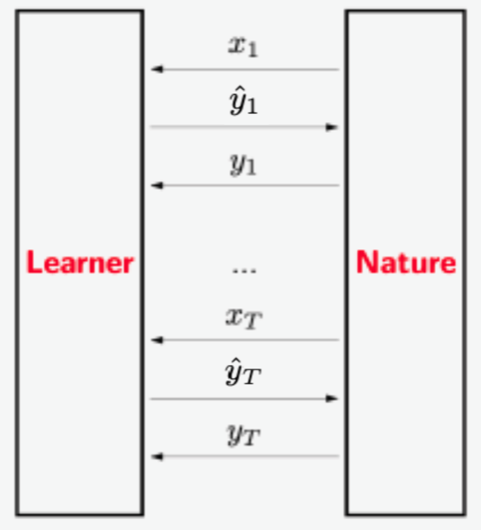
\includegraphics[width=2in]{figures/OLupdated.png}
    \caption{A representation of the online learning problem.}
    \label{lec15:fig:OLgame}
\end{figure}

Note that in online learning, it is possible that the ``true label'' $y_t$ is not generated at the same time as $x_t$. The environment could generate the label $y_t$ depending on the prediction $\hat{y}_t$ made by the learner. Later, we will see that the manner that nature generates  $(x_t, y_t)$ leads to different types of online learning. We can also see that Algorithm \ref{lec15:alg:gen-ol} is a very general framework as there are very few constraints on how $x_t$ and $y_t$ are generated.
    
\subsec{Evaluation of the learner}
Given this set-up, a natural question to ask is how one can evaluate the performance of the learner. Intuitively, one could simply evaluate the learner's performance by computing the loss between the predicted label and the ``true'' label sent by the environment $\ell(y_t, \hat{y}_t)$. For the entire sequence of tasks, one can then evaluate in terms of the cumulative loss:
    \begin{align}
        \sum_{t=1}^T \ell(y_t, \yhat_t).
    \end{align}
    
However, as the environment can be adversarial, the task itself might be inherently hard and even the best possible learner fails to achieve a small loss. For example, in a zero-one loss setting, the environment can always choose to select $y_t \neq \yhat$ for \textit{any} learner!

Hence, instead instead of using the cumulative loss for a learner by itself, we compare its performance against a suitable baseline, the ``best model in hindsight''. Assume that our learner comes from a set of hypotheses $\mathcal{H}$. Let us choose the hypothesis $h \in \mathcal{H}$ that minimizes the cumulative loss, i.e.
\begin{equation}
    h^* = \argmin_{h \in \mathcal{H}} \sum_{t=1}^T \ell(y_t, h(x_t)).
\end{equation}

Note here that in minimizing the cumulative loss, the learner gets to see all the data points $(x_t, y_t)$ at once. The cumulative loss of $h^*$ is the best we can ever hope to do, and so it would be better to compare the cumulative loss of the learner against it. (This approach is analogous to ``excess risk'', which tells how far the current model is away from the best we could hope for.) This measurement is denoted as \emph{regret}, and is formally defined as:
    \begin{align}
        \text{Regret} \overset{\Delta}{=} 
        \left[\sum_{t=1}^T \ell(y_t, \yhat_t)\right]
        - \underbrace{
        \left[\min_{h \in \mathcal{H}} \sum_{t=1}^T \ell(y_t, h(x_t))\right]
        }_{\text{best loss in hindsight}}
    \end{align}

Using this definition, if the best model in hindsight performs well, then the learner has more responsibility to learn to predict well in order to match up the performance of the baseline.
    
\subsec{The realizable case}
In general, if the environment is too powerful, leading the learner to a large loss, it will also hinder the best model in hindsight from doing well. On the other hand, there are settings where some members of the hypothesis class can actually do well. Such settings/problems are usually referred to as \textit{realizable}:

\begin{definition}[Realizable problem]
An online learning problem is \textit{realizable} (for a family of predictors $\mathcal{H}$) if there exists $h \in \mathcal{H}$ such that for any $T$, $\sum_{t = 1}^T \ell(y_t, h(x_t)) = 0$.
\end{definition}

Note that even though zero error is possible, this is still an interesting problem to consider because the $x_t$'s are not i.i.d. as they are in classical supervised learning. Hence, standard statistical learning theory does not apply, and there is still research to be done here.

\begin{example}
Consider a classification problem on $(x_t, y_t)$, and for simplicity assume $y_t \in \{0, 1\}$. Suppose there exists $h^* \in \mathcal{H}$ such that we always have $y_t = \yhat^*_t = h^*(x_t)$. In this case, the problem is realizable. 
    
In this case, the learner can adopt a ``majority algorithm''. At each time, the learner maintains a set $V_t \subset \mathcal{H}$ so that $\sum_{t=1}^T \ell (y_t, h(x_t)) = 0$ for all $h \in V_t$, and $\hat{y}_t$ is simply the prediction made by the majority of $h \in V_t$. Based on the loss received, learners $h \in V_t$ that fail for time $t + 1$ will be eliminated from future $V_t$'s.
    
With this setup, we can see that for each wrong prediction made by the learner, at least half of the hypotheses $h \in V_t$ will be eliminated. Hence, $1 \leq |V_{t+1}| \leq |\mathcal{H}|2^{-M}$ where $M$ is the number of mistakes made so far. Thus, one has $M \leq \log |\mathcal{H}|$ by taking log on both sides of inequalities and rearrange.
    
Now, if one puts $\ell$ as the zero-one loss, the regret for this example will be
\begin{equation}
\text{Regret} = \sum_{t=1}^T \ell(y_t, h(x_t)) = M,
\end{equation}
so in this example, one has $\text{regret} \leq \log |\mathcal{H}|$, which is a non-trivial bound when $\mathcal{H}$ is finite.
\end{example}
    
As one can see in the example, the realizable case usually indicates that the problem is not too far out of reach, and online learning is basically attempting to learn the $h \in \mathcal{H}$ that achieves the zero training loss. Hence, most literature focuses on non-realizable cases. However, the realizable case is still an interesting problem to consider because the $x_t$'s are not i.i.d. as they are in classical supervised learning. Hence, standard statistical learning theory does not apply, and there is still research to be done here.
 
To tackle this category of problems, we usually find reducing this problem to online optimization, which is a boarder problem scholars study on, helpful. This tool is our main focus in the next section.
    
\sec{Online (convex) optimization (OCO)}

\textit{Online convex optimization (OCO)} is a particularly useful tool to get results for online learning. Many online learning problems (and many other types of problems!) can be reduced to OCO problems, which allow them to be solved and analyzed algorithmically. Algorithm \ref{lec15:alg:oco} describes the OCO problem, which is more general than the online learning problem. (Note: \textit{Online optimization (OO)} refers to Algorithm \ref{lec15:alg:oco} except that the $f_t$'s need not be convex. However, due to the difficulty in non-convex function optimization, most research has focused on OCO.)

    \begin{algorithm}\label{lec15:alg:oco}
    \caption{Online (convex) optimization problem}
    \For{$t = 1, ..., T$} {
        The learner picks some action $w_t \in \Omega$ from the action space $\Omega$\;
        The environment picks a (convex) function $f_t: \Omega \to [0, 1]$\;
        The learner suffers the loss $f_t(w_t)$ and observes the \emph{entire} loss function $f_t(\cdot)$.
        }
    \end{algorithm}
    
Essentially the learner is trying to minimize the function $f_t$ at each step. As with online learning, one evaluates the performance of learner in online optimization setting using the regret:
\begin{align}
\text{Regret} = \sum_{t=1}^T f_t(w_t) - 
\underbrace{\min_{w \in \Omega} \sum_{t=1}^T f_t(w)}_\text{best action in hindsight}.
\end{align}

At some level, OCO seems like an impossible task, since we are trying to minimize a function $f_t$ that we only get to see \textit{after} we have made our prediction! This is certainly the case for $t = 1$. However, as time goes on, we see more and more functions and, if future functions are somewhat related to past functions, we have more information to make better predictions.

\subsec{Settings and variants of OCO}
There are multiple settings of the OCO network, which can vary the power of the environment and observations.

\begin{itemize}
    \item \underline{Stochastic setting:} $f_1,...,f_T$ are i.i.d samples from some distribution $P$. This corresponds to $(x_t, y_t)$ being i.i.d. in online learning. Under this setting, the environment is not adversarial.
    \item \underline{Oblivious setting:} $f_1,...,f_T$ are chosen arbitrarily but before the game starts. This corresponds to $(x_t, y_t$ being chosen before the game starts. In this setting, the environment can be adversarial but cannot be adaptive. The environment can choose these functions based on the learner's algorithm, but not the actual action if the learner's algorithm contains randomness. (This is the setting that we focus on in this course.)
    \item \underline{Non-oblivious/adaptive setting:} For all $t$, $f_t$ can depend on the learner's actions $w_1,...w_t$. Under this setting, the environment can be adversarial and adaptive. This is the most challenging setting because the environment is powerful enough to know not only the strategy of the learner, but also the exact choice the learner finally made. (Note however that If the learner is deterministic, the environment does not have more power here than in the oblivious setting. The oblivious adversary can simulate the game before the game starts, and chose the most adversarial input accordingly.)
\end{itemize}
 
\sec{Reducing online learning to online optimization}
There is a natural way to reduce the online learning problem to online optimization, with respect to a specific type of model $h_{w}$ parametrized by $w \in \Omega$. Recall that in online learning problem, the learner predicts $y_t$ upon receiving $x_t$. If the learner possesses oracle to solve online optimization problem, the learner can consult the oracle to obtain $w_t$, the parameter of the model as in online optimization problem, and then predict $\hat{y}_t = h_{w_t}(x_t)$.

In the next two subsections, we give two examples of how an online learning problem can be reduced to an OCO problem.
    
\subsec{Example: Online learning regression problem}

Consider the regression model $h_w(x) = w^\top x$ parameterized by $w$ in parameter space $\Omega$ with squared error loss $\ell$. Here is the online learning formulation of the regression problem:

\begin{algorithm}
\caption{Online learning regression problem}
\For{$t = 1, ..., T$} {
The learner receives $x_t \in \R^d$ from the environment\;
The learner predicts $\yhat_t$\;
The environment selects $y_t$ and sends it to the learner\;
The learner suffers loss $\ell(y_t, \yhat_t) = (y_t-\yhat_t)^2$.
}
\end{algorithm}

This can be reduced to the OCO problem in the following way:

\begin{algorithm}
\caption{OCO formulation of regression problem}
\For{$t = 1, ..., T$} {
The learner receives $x_t \in \R^d$ from the environment\;
The learner gives $x_t$ to the OCO solver and obtains $w_t \in \R^d$\;
The learner predicts $\hat{y}_t = h_{w_t}(x_t) = w_t^\top x_t$\;
The environment selects $y_t$ and sends it to the learner\;
The learner suffers loss $(y_t - h_{w_t}(x_t))^2$\;
With $(x_t, y_t)$ observed, the learner can reconstruct the loss function $f_t(w) = (y_t -h_{w}(x_t))^2$ and give it to the OCO solver.
}
\end{algorithm}

In this example, we have the following correspondence:
\begin{itemize}
\item $f_t$ in online optimization $\leftrightarrow$ squared error loss functions for $(x_t, y_t)$.
\item $w_t$ in online optimization $\leftrightarrow$ parameters of the linear model $h_{w_t}$.
\end{itemize}
    
Since $h_w(\cdot)$ is linear, the corresponding squared error loss function $f_t$ are convex, and so we have effectively reduced the online linear regression problem to an online \emph{convex} optimization problem.
    
Notice that in the previous example, the loss function $f_t$ actually depends on the label $y_t$, which demonstrates that the key challenge in online optimization is that the function $f_t$ is unknown to the learner when the prediction $\hat{y}_t$ is made.
    
\subsec{Example: The expert problem}
Suppose we wish to predict tomorrow's weather and 10 different TV channels provide different forecasts. Which one should we follow? Formally, consider a finite hypothesis class $\mathcal{H}$, where each $h \in \mathcal{H}$ represents an expert, and we wish to choose a $h_t$ wisely at each time step. For simplicity, we assume the prediction is binary, i.e. $\hat{y} \in \{0, 1\}$, and suppose the loss function is 0-1 loss. (The problem can easily be generalized to more general predictions and losses.) The problem is outlined in Algorithm \ref{lec15:alg:expert_discrete}.

\begin{algorithm}[h]
\caption{The expert problem}
\label{lec15:alg:expert_discrete}
\For{$t = 1, ..., T$}{
The learner obtains predictions from $N$ experts\;
The learner chooses to follow prediction of one of the experts $i_t \in [N]$\;
The environment gives the learner the true value. The learner is thus able to learn the loss of each of the experts: $\ell_t \in \{0, 1\}^N$\;
The learner suffers the loss of the expert which was chosen: $\ell_t(i_t)$.
}
\end{algorithm}

We want to design a method that chooses $i_t$ for each step (line 3 in Algorithm \ref{lec15:alg:expert_discrete}) to minimize the regret:
\begin{equation}
\text{Regret} \overset{\Delta}{=} \mathbb{E}\left[
\sum_{t=1}^T \ell_t(i_t)
- \underbrace{\min_{i \in [N]} \sum_{t=1}^T \ell_t(i)}_\text{the best expert in hindsight}
\right],
\end{equation}
where the expected value is over $i_t$, thus covering the case where the $i_t$'s could be random.
    
To make the expert problem amenable to reduction to OCO, we introduce idea of a \textit{continuous action space}. Instead of choosing $i_t$ from $\Omega = [N]$, the learner chooses a distribution $p_t$ from the $N$-dimensional simplex $\Delta(N) = \left\{p \in \R^N : \norm{p}_1 = 1, p \geq 0 \right\}$. The learner then samples $i_t \sim p_t$. With this formulation, instead of selecting particular expert $i_t$ to follow, the learner adjusts the belief $p_t$, and samples from the distribution to choose which expert to follow. Algorithm \ref{lec15:alg:expert_randomized} outlines this procedure. Note that the loss is the expected loss $\mathbb{E}_{i \sim p_t}[\ell_t(i)]$ instead of the sampled $\ell_t(i_t)$.

\begin{algorithm}
\caption{The expert problem with continuous action}
\label{lec15:alg:expert_randomized}
\For{$t = 1, ..., T$}{
The learner obtains predictions from $N$ experts\;
The learner chooses a distribution $p_t \in \Delta(N)$\;
The learner samples one expert $i_t \sim p_t$\;
The environment gives the learner the true value and the loss/error of all experts: $\ell_t \in \{0, 1\}^N$\;
The learner suffers expected loss $\sum_{i\in[N]} p_t(i) \ell_t(i) = \langle p_t, \ell_t \rangle$\;
}
\end{algorithm}
    
With the continuous action space, it is easy to reduce the expert problem to an OCO: see Algorithm \ref{lec15:alg:expert_discrete_oco}. (The problem is convex since the loss function is convex and the parameter space $\Delta(N)$ is convex.)

\begin{algorithm}[h]
\caption{The expert problem}
\label{lec15:alg:expert_discrete_oco}
\For{$t = 1, ..., T$}{
The learner obtains predictions from $N$ experts\;
The learner invokes the OCO oracle to obtain $p_t \in \Delta(N)$\;
The learner chooses to follow prediction of one of the experts $i_t \in [N]$\;
The environment gives the learner the true value. The learner is thus able to learn the loss of each of the experts: $\ell_t \in \{0, 1\}^N$\;
The learner suffers the loss of the expert which was chosen: $\ell_t(i_t)$.
The learner can reconstruct the loss function $f_t (p) = \langle p, \ell_t \rangle$ and give it to the OCO oracle.
}
\end{algorithm}

In this setting, one can rewrite the regret as:
\begin{align}
\text{Regret} &= \sum_{t=1}^T \langle p_t, \ell_t \rangle - \min_{i\in[N]}\sum_{t=1}^T \ell_t(i)  \\
&= \sum_{t=1}^T \langle p_t, \ell_t \rangle - \min_{p \in \Delta(N)}\sum_{t=1}^T \langle p, \ell_t \rangle \label{lec15:eqn:changearg} \\
&= \sum_{t=1}^T f_t(p_t) - \min_{p \in \Delta(N)}\sum_{t=1}^T f_t(p). \label{lec15:eqn:regret}
\end{align}

We obtain \eqref{lec15:eqn:changearg} because
\begin{align}
\sum_{t=1}^T \langle p, \ell_t \rangle &=  \left\langle p,  \sum_{t=1}^T\ell_t \right\rangle \geq \min_{i \in [N]} \left[ \sum_{t=1}^T \ell_t (i) \right],
\end{align}
with equality for the probability distribution $p(i) =1$ when $i = \text{argmin}_i \left[ \sum_{t=1}^T \ell_t (i) \right]$ and $p(i) = 0$ otherwise, and \eqref{lec15:eqn:regret} is by definition of $f_t$.


\sec{Reducing online learning to batch learning}    
In this section, we present a reduction from online learning to standard supervised learning problem, also known as the ``batch problem'' in this literature.

As in the standard supervised learning setting, consider an i.i.d dataset $\{(x_t, y_t)\}_{t=1}^T$ and some parameter $w$. Let $L(w)$ and $\hatL(w)$ be the population loss and empirical loss respectively. For simplicity, assume $|\ell((x_i, y_i), w)| \leq 1$. The theorem below establishes a link between the regret obtained in online learning and the excess risk obtained in the batch setting.
    
\begin{theorem}[Relationship between excess risk and regret]
Assume $\ell((x, y), w)$ is convex. Suppose we run an online learning algorithm on the dataset $\{(x_i, y_i)\}_{i=1}^T$ and obtain a sequence of models $w_1, \dots, w_T$, and regret $R_T$. Let $\overline{w} = \frac{1}{T} \sum_{i=1}^T w_i$, then the excess risk of $\overline{w}$ can be bounded above:
\begin{align}
L(\overline{w}) - L(w^*) \leq \frac{R_T}{T} + \tilO\left(\frac{1}{\sqrt{T}}\right), \label{lec15:eqn:lec15_ol_gen_bound}
\end{align}
where $w^* = \argmin_{w \in \Omega} L(w)$.
\end{theorem}

Here are some intuitive interpretations of the theorem:

    \begin{itemize}
        \item If $R_T = O(T)$, then we have some non-trivial result. Otherwise, the bound in \eqref{lec15:eqn:lec15_ol_gen_bound} is increasing $T$ and does not provide any useful information.
        \item If the batch problem has a $1 / \sqrt{T}$ generalization bound, then the best you can hope for in online learning is $R_T = O(\sqrt{T})$.
        \item If the batch problem has a $1 / T$ generalization bound, you can hope for $O(1)$ regret (or $\tilO(1)$ regret in some cases).
        \item We often have $O(\sqrt{T})$ excess risk supervised learning problems; hence it is reasonable to expect $O(\sqrt{T})$ regret in online learning problems.
    \end{itemize}
    
\sec{Follow-the-Leader (FTL) algorithm} \label{lec15:sec:FTL}
In this section, we analyze an algorithm called ``Follow-the-Leader'' (FTL) for OCO, which is intuitive but fails to perform well in many cases.

The FTL algorithm behaves as its name suggests: it always selects the action $w_t$ such that it minimizes the historical loss the learner has seen so far, i.e.
\begin{equation}
w_t = \argmin_{w \in \Omega} \sum_{i=1}^{t-1} f_i(w).
\end{equation}

We now demonstrate how the FTL algorithm can fail for the expert problem. In the expert problem, $f_t(p) = \langle p, \ell_t \rangle$, so 
    \begin{align}
        p_t &= \argmin_{p \in \Delta(N)} \sum_{i=1}^{t-1} f_i(p) \\
        &= \argmin_{p \in \Delta(N)} \sum_{i=1}^{t-1} \langle\ell_i, p\rangle \\
        &= \argmin_{p \in \Delta(N)} \left\langle\sum_{i=1}^{t-1}\ell_i, p\right\rangle.
    \end{align}

The minimizer $p \in \Delta(N)$ is a point-mass probability, with the point mass at the smallest coordinate of $\sum_{i=1}^{t-1} \ell_i$. This gives regret
\begin{equation}
\text{Regret} = \sum_{i=1}^{t-1} \ell_i(i_t),
\quad \text{ where } i_t = \argmin_{j \in [N]} \sum_{i=1}^{t-1}\ell_i(j).
\end{equation}
    
Now, consider the following example: suppose we have only two experts. Suppose expert 1 makes perfect predictions on even days while expert 2 makes perfect predictions on odd days. Assume also that the FTL algorithm chooses expert 1 to break ties (this is not an important point but makes the exposition simpler.) In this setting, the FTL algorithm always selects the \textit{wrong} expert to follow. A few rounds of simulation of this example is shown in Table \ref{lec15:tab:counter example}.

    \begin{table}[h]
        \caption{An example where FTL fails}
        \label{lec15:tab:counter example}
        \medbreak
        \centering
        \small
        \begin{tabular}{l|c c c c c c}
        \toprule
        Day & 1 & 2 & 3 & 4 & $\dots$ & $\dots$ \\
        \midrule 
        Expert 1's loss & 1 & 0 & 1 & 0 & $\dots$ & $\dots$ \\
        Expert 2's loss & 0 & 1 & 0 & 1 & $\dots$ & $\dots$ \\
        \midrule 
        \midrule 
        FTL choice $i_t$ & 1 & 2 & 1 & 2 & 1 & $\dots$ \\
        \bottomrule
        \end{tabular}
    \end{table}

The best expert in hindsight has a loss of $T/2$ (choosing either expert all the time incurs this loss, and so the regret of the FTL algorithm is $T - T/2 = T/2 = \Theta(T)$. The main reason for FTL's failure is that is a deterministic algorithm driven by an extreme update, with no consideration on potential domain shift (it always selects the best expert based on the past with no consideration of the potential next $f_t$). Knowing its deterministic strategy, the environment can easily play in an adversarial manner. To perform better in a problem like this, we need some randomness to hedge risk.